\documentclass[a4paper,10pt]{article}
%ArXiv allows 10pt - 14pt

\usepackage{publication}
\usepackage[backend=biber]{biblatex}
\addbibresource{references.bib}
\usepackage{float} % Needed for the [H] float option
\usepackage{graphicx}

% Title formatting
\title{Simple Documentación del Pipeline}

\author[1]{TFG}
\contact{\dots @fpuna.edu.py}
\affil[1]{FPUNA}


%\keywords{Keyword 1, Keyword 2, Keyword 3}
\date{\today}

\begin{document}

\maketitle

\begin{abstract}
En el presente proyecto se aborda el problema de la predicción del riesgo de incendios forestales en el Departamento de Cordillera, Paraguay, haciendo uso de un pipeline automatizado de procesamiento de datos geoespaciales y un modelo avanzado de Machine Learning. El marco temporal del estudio se define en función del histórico de datos de focos de calor provistos por el sistema FIRMS de la NASA.

Se integran múltiples variables predictoras correspondientes a categorías topográficas (elevación, pendiente, orientación), meteorológicas (temperatura, precipitación, viento, humedad), de vegetación (NDVI), de cobertura del suelo y de proximidad a infraestructuras humanas (distancia a vías y ciudades). Para la generación de la muestra, se utilizan los puntos de focos de calor como observaciones positivas y se implementa una estrategia de muestreo de fondo espacio-temporal para generar observaciones negativas (no-incendio) de alta calidad, evitando el sesgo de un muestreo puramente aleatorio.

Se genera una muestra final balanceada que se utiliza para entrenar y evaluar el modelo. Críticamente, para evitar una evaluación sesgada por la autocorrelación espacial, se emplea una validación por bloques espaciales en lugar de una partición aleatoria. El modelo central implementado es un \texttt{StackingClassifier}, un método de ensamble que combina las predicciones de varios estimadores base (Random Forest, Support Vector Machine y k-Nearest Neighbours) a través de un meta-modelo de Regresión Logística para mejorar la robustez y precisión predictiva.

Se evalúa el rendimiento del modelo sobre un conjunto de prueba geográficamente aislado, utilizando métricas clave como Accuracy, ROC AUC, la matriz de confusión y el reporte de clasificación. El modelo de ensamble demuestra un rendimiento prometedor en la distinción entre condiciones de incendio y no-incendio. Finalmente, el pipeline culmina con la aplicación del modelo entrenado para generar un mapa de riesgo de alta resolución para una fecha específica, proporcionando una herramienta visual e interpretable para la gestión y mitigación de incendios en la región.
\end{abstract}


\begin{multicols}{2}

\section{Librerías}
\subsection{Manipulación y Análisis de Datos Fundamentales}
\begin{itemize}
    \item \textbf{pandas:} (import pandas as pd) librería principal para la manipulación y el análisis de datos estructurados. Se utilizó para leer los archivos .csv que contienen los focos de calor (FIRMS) y los datos climáticos (temperatura, precipitación, etc.). Permitió combinar estas diferentes fuentes de datos, manejar las series temporales con la columna date, y organizar toda la información en un formato de DataFrame, que es la estructura de datos central a lo largo de todo el proyecto.
    \item \textbf{numpy:} (import numpy as np) paquete fundamental para la computación numérica. Se empleó para fijar las semillas aleatorias (np.random.seed) garantizando la reproducibilidad de los resultados. También se usó para generar los puntos aleatorios de la muestra negativa y para crear la rejilla (meshgrid) sobre la que se genera el mapa de riesgo final. Muchas otras librerías, como pandas y scikit-learn, dependen de numpy para sus operaciones internas.
\end{itemize}
\subsection{Manejo de Datos Geoespaciales (Vectoriales y Raster)}
\begin{itemize}
    \item \textbf{geopandas:} (import geopandas as gpd) extiende pandas para permitir el trabajo con datos geoespaciales vectoriales. Utilizado para leer los archivos de forma (.shp) del departamento, distritos, ciudades y vías. Permitió convertir las coordenadas de los incendios en objetos geométricos (\texttt{points\_from\_xy}), filtrar los puntos que caen dentro del área de estudio (\texttt{.within}), y calcular distancias a elementos geográficos como vías y ciudades (\texttt{.distance}). También se usó para visualizar las capas vectoriales en los mapas.
    \item \textbf{shapely.geometry.Point:} (from shapely.geometry import Point) Proporciona los objetos geométricos que geopandas utiliza. Se usó directamente para crear objetos Point a partir de coordenadas aleatorias durante la generación de las muestras negativas, antes de convertirlas a un GeoDataFrame.
    \item \textbf{rasterio:} (import rasterio) Es la librería principal para leer, escribir y manipular datos geoespaciales en formato raster (como archivos \texttt{.tif}). Se utilizó para abrir y leer los datos del Modelo Digital de Elevación (DEM) y los mapas de cobertura del suelo. La función \texttt{rasterio.features.shapes} fue clave para vectorizar las clases de cobertura inflamables, convirtiendo píxeles del raster en polígonos que definen las "zonas inflamables".
    \item \textbf{rioxarray:} Actúa como un puente entre rasterio y xarray, facilitando operaciones complejas en datos raster. Se usó para abrir los archivos raster \texttt{(.tif)} de DEM, Cobertura y NDVI como DataArrays de xarray. Su función más importante en el script fue la reproyección \texttt{(.rio.reproject())} del DEM a un sistema de coordenadas métrico (UTM), un paso indispensable para calcular correctamente la pendiente y la orientación.
    \item \textbf{xarray:} (xr) Permite trabajar con arreglos N-dimensionales etiquetados, ideal para los rasters. Se utilizó para crear DataArrays a partir de las coordenadas de los puntos. Su método de selección basado en etiquetas \texttt{(.sel(method="nearest"))} fue fundamental para extraer de manera eficiente los valores de los rasters (elevación, pendiente, NDVI, etc.) correspondientes a la ubicación de cada punto de la muestra.
    \item \textbf{xrspatial:} (xrs) es una extensión de xarray para análisis espaciales basados en rasters. Se utilizó para calcular las variables topográficas de pendiente (xrs.slope()) y orientación (xrs.aspect()) a partir del DEM reproyectado.
\end{itemize}
\subsection{Modelado Predictivo y Evaluación (Machine Learning)}
\begin{itemize}
    \item \textbf{scikit-learn (sklearn):} librería utilizado para realizar tareas de aprendizaje automático supervisado y no supervisado.
    \begin{itemize}
        \item \textbf{-preprocessing:} Se usó StandardScaler para normalizar las variables numéricas (como elevación o temperatura) y OneHotEncoder para convertir las variables categóricas (como el tipo de cobertura) en un formato numérico que el modelo pueda procesar.
        \item \textbf{-compose.ColumnTransformer:} Permitió aplicar los diferentes pasos de preprocesamiento (escalado y codificación) a las columnas correspondientes de forma organizada. 
        \item \textbf{-pipeline.Pipeline:} Se utilizó para encadenar el preprocesador y el modelo clasificador en un único objeto. Esto asegura que el mismo procesamiento se aplique de forma consistente a los datos de entrenamiento, prueba y predicción, evitando errores y fugas de datos.
        \item -ensemble.RandomForestClassifier, svm.LinearSVC,
        
        neighbors.KNeighborsClassifier: Estos fueron los tres modelos base utilizados en el ensamble.
        \item \textbf{-ensemble.StackingClassifier:} Fue el núcleo del modelado, permitiendo combinar las predicciones de los tres modelos base para obtener un resultado final más preciso y robusto.
        \item \textbf{-linear\_model.LogisticRegression:} Se usó como el meta-modelo dentro del StackingClassifier, encargado de aprender a combinar las predicciones de los modelos base.
        \item \textbf{-calibration.CalibratedClassifierCV:} Se usó para envolver al LinearSVC, ya que este último no produce probabilidades de forma nativa. Este calibrador le permite generar las estimaciones de probabilidad necesarias para el StackingClassifier y el cálculo del AUC-ROC.
        \item \textbf{-metrics:} Se usaron funciones como \texttt{accuracy\_score}, \texttt{confusion\_matrix}, \texttt{classification\_report} y \texttt{roc\_auc\_score} para realizar una evaluación exhaustiva del rendimiento del modelo final.
    \end{itemize}
\end{itemize}
\subsection{Explicabilidad e Interpretación del Modelo}
\begin{itemize}
    \item \textbf{shap:} Se utilizó para explicar las predicciones del modelo RandomForest. Se creó un TreeExplainer para calcular los valores SHAP, que miden el impacto de cada variable en la predicción. Con ellos se generaron los gráficos de resumen (summary\_plot) que visualizan qué variables son las más importantes y cómo influyen en el riesgo de incendio.
\end{itemize}
\subsection{Visualización de Datos y Resultados}
\begin{itemize}
    \item \textbf{matplotlib.pyplot:} Es la librería fundamental para crear todo tipo de gráficos y visualizaciones. Se utilizó para crear la estructura de todas las figuras, configurar títulos, ejes, guardar los gráficos en archivos (.png) y mostrarlos en pantalla.
    \item \textbf{seaborn:} Construida sobre matplotlib, facilita la creación de gráficos estadísticos más complejos y estéticamente agradables. Se usó para generar los diagramas de caja (boxplot) que comparan las distribuciones de las variables entre los casos de incendio y no-incendio, y para crear el mapa de calor (heatmap) de la matriz de confusión.
    \item \textbf{scipy.interpolate.griddata:}  función de la librería científica SciPy esencial para crear el mapa de riesgo final. Interpoló las probabilidades de incendio predichas en puntos dispersos para crear una superficie continua y suave (un heatmap), que es mucho más fácil de interpretar visualmente.
    \item \textbf{contextily:} utilizadp para agregar un mapa de fondo a las visualizaciones espaciales (cx.add\_basemap), lo que proporciona un contexto geográfico invaluable para entender dónde se localizan los puntos de la muestra y las zonas de alto riesgo.
    \item \textbf{matplotlib.patches y matplotlib.path:}  Módulos para crear formas y trazados complejos. Se utilizaron para crear una máscara de recorte a partir del polígono del departamento. Esto permitió que el mapa de calor interpolado se mostrara únicamente dentro de los límites del área de estudio.
\end{itemize}
\subsection{Librerías Estándar de Python}
\begin{itemize}
    \item \textbf{os:} Proporciona funciones para interactuar con el sistema operativo. Para establecer una variable de entorno (PYTHONHASHSEED) con el fin de mejorar la reproducibilidad.
    \item \textbf{datetime:}  para trabajar con fechas y horas  y así crear un nombre de carpeta único (TIMESTAMP) donde guardar todos los resultados de una ejecución.
    \item \textbf{pathlib.Path:} Se utilizó de forma extensiva para definir todas las rutas a los datos de entrada y a las carpetas de salida.
    \item \textbf{shutil:} para copiar los resultados más importantes (mapas, reportes) desde la carpeta de salida con timestamp a una carpeta fija (frontend/ouput), preparándolos para ser consumidos por una aplicación web o dashboard.
    \item \textbf{io:} para capturar la salida de texto del resumen del DataFrame (.info()) como una cadena de texto, para luego guardarla en un archivo.
\end{itemize}


\section{Funciones Auxiliares}
\subsection{Función \texttt{load\_firms\_data}}

\begin{itemize}
    \item \textbf{Propósito:} Cargar, filtrar y formatear los datos de focos de calor del sistema FIRMS (Fire Information for Resource Management System).

    \item \textbf{Parámetros:}
    \begin{itemize}
        \item \texttt{firms\_folder}: Ruta a la carpeta que contiene los archivos \texttt{.csv} con los datos de focos de calor.
        \item \texttt{study\_area\_geom}: Objeto de geometría poligonal que define los límites del área de estudio (el departamento de Cordillera).
        \item \texttt{crs}: Sistema de Coordenadas de Referencia (CRS) del área de estudio, para asegurar la coherencia espacial.
    \end{itemize}

    \item \textbf{Proceso:}
    \begin{enumerate}
        \item Localiza y lee todos los archivos \texttt{.csv} dentro de la carpeta especificada y los combina en un único \texttt{DataFrame} de \texttt{pandas}.
        \item Convierte la columna de fecha (\texttt{acq\_date}) a formato \texttt{datetime}.
        \item Transforma el \texttt{DataFrame} en un \texttt{GeoDataFrame} de \texttt{geopandas}, usando las columnas de latitud y longitud.
        \item Filtra espacialmente: descarta todos los puntos fuera del polígono del área de estudio.
        \item Añade una columna \texttt{fire} con el valor \texttt{1}, etiquetando estos puntos como positivos (presencia de incendio).
        \item Devuelve solo las columnas esenciales: fecha, geometría y etiqueta.
    \end{enumerate}

    \item \textbf{Retorno:} Un \texttt{GeoDataFrame} que contiene exclusivamente los focos de calor ocurridos dentro del área de estudio, listo para ser usado como muestra positiva.
\end{itemize}

\subsection{Función \texttt{load\_climate\_data}}

\begin{itemize}
    \item \textbf{Propósito:} Cargar y unificar los diferentes archivos de datos climáticos en una única serie temporal diaria.

    \item \textbf{Parámetros:}
    \begin{itemize}
        \item \texttt{temp\_path}, \texttt{precip\_path}, \texttt{wind\_path}, \texttt{humidity\_path}: Rutas a los archivos \texttt{.csv} de temperatura, precipitación, viento y humedad.
    \end{itemize}

    \item \textbf{Proceso:}
    \begin{enumerate}
        \item Carga cada archivo de forma independiente, selecciona y renombra columnas.
        \item Combina los \texttt{DataFrames} de temperatura, precipitación y viento.
        \item Aplica \texttt{resample} para convertir a escala diaria: media para temperatura y viento, suma para precipitación.
        \item Fusiona el \texttt{DataFrame} diario con los datos de humedad.
        \item Rellena valores faltantes usando \texttt{ffill().bfill()}.
    \end{enumerate}

    \item \textbf{Retorno:} Un \texttt{DataFrame} indexado por fecha con datos climáticos diarios completos para las cuatro variables.
\end{itemize}

\subsection{Función \texttt{asignar\_variables}}

\begin{itemize}
    \item \textbf{Propósito:} Asignar variables predictoras a un conjunto de puntos a partir de fuentes de datos raster y vectoriales.

    \item \textbf{Parámetros:}
    \begin{itemize}
        \item \texttt{df\_puntos}: El \texttt{GeoDataFrame} de puntos (incendio o no).
        \item \texttt{dem\_path}, \texttt{cobertura\_folder}, \texttt{ndvi\_mensual\_folder}: Rutas a los datos raster.
        \item \texttt{weather\_df}: \texttt{DataFrame} de clima diario desde \texttt{load\_climate\_data}.
        \item \texttt{vias\_shp\_path}, \texttt{ciudades\_shp\_path}: Archivos de forma para el cálculo de distancias.
    \end{itemize}

    \item \textbf{Proceso:}
    \begin{enumerate}
        \item \textbf{Topografía:}
        \begin{itemize}
            \item Extrae la elevación desde el DEM.
            \item Reproyecta el DEM a CRS métrico para calcular pendiente y orientación (usando \texttt{xrspatial}).
            \item Convierte la orientación a categorías cardinales.
        \end{itemize}
        \item \textbf{Cobertura del suelo:}
        \begin{itemize}
            \item Itera por año y extrae la clase de cobertura correspondiente para cada punto.
        \end{itemize}
        \item \textbf{Vegetación (NDVI):}
        \begin{itemize}
            \item Para cada punto, extrae el valor del raster NDVI mensual correspondiente al mes y año.
        \end{itemize}
        \item \textbf{Clima:}
        \begin{itemize}
            \item Asigna los valores climáticos del día correspondiente usando \texttt{merge\_asof}.
        \end{itemize}
        \item \textbf{Proximidad:}
        \begin{itemize}
            \item Reproyecta a CRS métrico.
            \item Calcula distancia a vías principales (\texttt{dist\_vias}) y a la ciudad más cercana (\texttt{dist\_ciudades}).
        \end{itemize}
    \end{enumerate}

    \item \textbf{Retorno:} El mismo \texttt{GeoDataFrame}, enriquecido con todas las variables predictoras necesarias para el modelado.
\end{itemize}
\section{Generación de la muestra y asingación de datos}
 Esta fase del script se encarga de construir el conjunto de datos que servirá de base para todo el análisis. El proceso se divide en \textbf{tres pasos principales}: la preparación del área de estudio y las muestras positivas, la generación de muestras negativas y, finalmente, la consolidación y enriquecimiento del conjunto de datos.
\subsection{Preparación del Área de Estudio y Muestras Positivas (Incendios)}

\begin{enumerate}
    \item \textbf{Carga del Área de Estudio:} El proceso comienza cargando el archivo de forma (\texttt{.shp}) del departamento de Cordillera. La geometría y el Sistema de Coordenadas de Referencia (CRS) de este polígono (\texttt{area\_estudio\_gdf}) se convierten en la referencia espacial para todo el análisis, asegurando que todos los datos subsiguientes estén geográficamente alineados.

    \item \textbf{Identificación de Zonas Inflamables:} Se implementa una optimización crucial para mejorar la calidad de la muestra. Utilizando un mapa de cobertura del suelo como referencia, se identifican las clases que se consideran ``inflamables'' (por ejemplo, pastizales, bosques). Estos píxeles se convierten en un único polígono (\texttt{zonas\_inflamables\_poligono}). Este polígono actúa como una máscara, asegurando que el modelo se enfoque únicamente en las áreas donde un incendio es plausible.

    \item \textbf{Carga de Puntos Positivos:} Se invoca la función \texttt{load\_firms\_data} para cargar los datos de focos de calor. Esta función lee los archivos \texttt{.csv} de FIRMS, los convierte en un \texttt{GeoDataFrame} y filtra únicamente aquellos puntos que caen dentro de los límites del departamento de Cordillera. Estos puntos, etiquetados con \texttt{fire = 1}, constituyen la muestra positiva, es decir, los casos confirmados de incendios que el modelo aprenderá a predecir.
\end{enumerate}

\subsection{Generación de Muestras Negativas (No-Incendios)}

No existe un registro de ``lugares donde no hubo un incendio'', por ello es necesario generar una muestra sintética de puntos negativos. El script emplea una estrategia de \textbf{muestreo de fondo inteligente} para crear puntos negativos realistas para el modelo.

\begin{enumerate}
    \item \textbf{Balance de Clases:} Se decide generar un número de puntos negativos igual al de puntos positivos, creando un conjunto de datos perfectamente balanceado.

    \item \textbf{Proceso de Generación Iterativo:} Se inicia un bucle que genera puntos aleatorios uno por uno hasta alcanzar el número deseado. Cada punto candidato debe pasar una serie de filtros rigurosos para ser aceptado:

    \begin{itemize}
        \item \textbf{Filtro Espacial Primario:} El punto debe caer no solo dentro de los límites del departamento, sino también \textbf{dentro del polígono de zonas inflamables} previamente creado. Esto evita generar puntos ``fáciles'' en lugares como cuerpos de agua o centros urbanos densos donde un incendio forestal es imposible.

        \item \textbf{Filtro Espacio-Temporal:} Para evitar que un punto negativo esté demasiado cerca de un incendio real (cosa que podría confundir al modelo), se aplica una restricción de proximidad. A cada punto candidato se le asigna una \textbf{fecha aleatoria} dentro del rango de estudio. Luego, se comprueba que no exista ningún incendio real en un radio de \textbf{15 kilómetros} y en una ventana temporal de \textbf{3 días} (antes y después) de esa fecha.
    \end{itemize}

    Solo si un punto candidato supera ambos filtros, se añade a la lista de puntos negativos (\texttt{puntos\_negativos\_list}) y se le asigna la etiqueta \texttt{fire = 0}.
\end{enumerate}

\subsection{Consolidación y Asignación de Variables Predictoras}

\begin{enumerate}
    \item \textbf{Combinación y Aleatorización:} Una vez generados los puntos negativos, se convierten en un \texttt{GeoDataFrame}. Este se concatena con el \texttt{GeoDataFrame} de puntos positivos. El conjunto de datos resultante (\texttt{sample}) se mezcla de forma aleatoria (\texttt{.sample(frac=1)}) para asegurar que los casos positivos y negativos no estén agrupados, lo cual es crucial para el entrenamiento del modelo.

    \item \textbf{Carga de Datos Climáticos:} Se llama a la función \texttt{load\_climate\_data} para obtener la serie temporal diaria de variables meteorológicas (temperatura, precipitación, viento y humedad).

    \item \textbf{Enriquecimiento del Conjunto de Datos:} Finalmente, se invoca la función principal de ingeniería de características, \texttt{asignar\_variables}. Esta función toma el \texttt{GeoDataFrame} combinado de puntos positivos y negativos y, para cada punto, extrae y asigna todas las variables predictoras:

    \begin{itemize}
        \item \textbf{Topográficas:} Elevación, pendiente y orientación.
        \item \textbf{Vegetación:} Cobertura del suelo y NDVI.
        \item \textbf{Climáticas:} Temperatura, precipitación, humedad y viento correspondientes a su fecha.
        \item \textbf{Antropogénicas:} Distancia a vías principales y ciudades.
    \end{itemize}
\end{enumerate}

El resultado de esta fase es el \texttt{full\_dataset}, un \texttt{GeoDataFrame} completo y enriquecido que contiene tanto las observaciones (puntos de incendio y no-incendio) como todas las variables predictoras necesarias, listo para ser depurado y utilizado en la fase de modelado.

\section{Depuración y Modelado Predictivo}
Esta fase se divide en dos etapas críticas: la depuración de los datos para asegurar su calidad y el proceso de modelado, que incluye una estrategia de validación espacialmente consciente.

\subsection{Depuración del Conjunto de Datos}

\begin{enumerate}
    \item \textbf{Detección de Nulos:} Se realiza un diagnóstico para identificar cuántos valores faltantes existen en cada columna del \texttt{full\_dataset}.
    
    \item \textbf{Estrategia de Eliminación:} se eliminan todas las filas (\texttt{.dropna()}) que contengan al menos un valor nulo. Aunque esto puede reducir el tamaño total de la muestra, garantiza que cada observación que ingresa al modelo sea completa, evitando errores y sesgos potenciales. Se realiza una comprobación para asegurar que, después de la depuración, quede un número suficiente de registros para un entrenamiento significativo.

    \item \textbf{Preparación del \texttt{DataFrame} Final:}
    \begin{itemize}
        \item Se crea un nuevo \texttt{DataFrame} llamado \texttt{datos\_modelo} que contiene exclusivamente las columnas que se utilizarán como variables predictoras y la variable objetivo (\texttt{fire}).
        \item Se convierte la columna \texttt{cobertura} al tipo de dato \texttt{category}, optimizando el uso de memoria y facilitando el tratamiento como variable categórica en \texttt{scikit-learn}.
        \item Finalmente, se guarda un resumen (\texttt{.info()}, \texttt{.head()}) del \texttt{DataFrame} final en un archivo de texto (\texttt{dataset\_summary.txt}), asegurando la \textbf{reproducibilidad} del análisis.
    \end{itemize}
\end{enumerate}

\subsection{Modelado con Validación Cruzada Espacial}

\begin{enumerate}
     \item \textbf{Autocorrelación Espacial:} Los datos geográficos tienen una propiedad inherente: los puntos cercanos en el espacio tienden a ser más similares entre sí. Si se utilizara una división aleatoria estándar (\texttt{train\_test\_split}), se correría el riesgo de que el conjunto de prueba contenga puntos muy similares a los del entrenamiento, inflando artificialmente la precisión del modelo.

    \item \textbf{División Espacial por Bloques:} Se implementa una \textbf{validación cruzada espacial}. En lugar de una división aleatoria, el departamento se divide geográficamente: el 70\% de los datos ubicados en el sur (según su latitud) se utilizan para \textbf{entrenar} el modelo, y el 30\% restante, ubicado en el norte, se reserva para \textbf{evaluarlo}. Esta estrategia simula un escenario realista, donde el modelo debe generalizar a una región completamente nueva, proporcionando una medida más honesta del rendimiento.

    \item \textbf{Pipeline de Preprocesamiento:} Se construye un \texttt{Pipeline} de \texttt{scikit-learn} para automatizar la preparación de los datos, asegurando consistencia entre entrenamiento y prueba.
    
    \begin{itemize}
        \item \texttt{StandardScaler}: Se aplica a todas las variables numéricas (elevación, temperatura, etc.), normalizándolas con media 0 y desviación estándar 1.
        \item \texttt{OneHotEncoder}: Se aplica a las variables categóricas (\texttt{orientacion\_cat} y \texttt{cobertura}), transformándolas en columnas binarias para permitir el procesamiento por modelos numéricos.
    \end{itemize}

    \item \textbf{Arquitectura del Modelo:} StackingClassifier: \textbf{Stacking}.
    
    \begin{itemize}
        \item \textbf{Estimadores Base:} Se definen tres clasificadores distintos:
        \begin{itemize}
            \item \texttt{RandomForestClassifier}
            \item \texttt{LinearSVC} calibrado
            \item \texttt{KNeighborsClassifier}
        \end{itemize}
        Cada uno aprende de manera independiente a partir del conjunto de entrenamiento.

        \item \textbf{Meta-Modelo:} Se define una \texttt{LogisticRegression} como meta-modelo, que aprende a combinar las predicciones de los modelos base. Esto para ofrecer una mejor capacidad predictiva al aprovechar las fortalezas individuales de cada clasificador.
    \end{itemize}

    \item \textbf{Entrenamiento y Evaluación:}
    \begin{itemize}
        \item El \texttt{Pipeline} completo (preprocesamiento + stacking) se entrena con el conjunto de entrenamiento espacial (\texttt{X\_train}, \texttt{y\_train}).
        \item Luego se evalúa en el conjunto de prueba espacial (\texttt{X\_test}, \texttt{y\_test}), que representa una región no vista por el modelo.
        \item Se calculan métricas clave como:
        \begin{itemize}
            \item \textbf{Accuracy}: Porcentaje total de aciertos.
            \item \textbf{ROC AUC Score}: Capacidad del modelo para distinguir entre clases.
            \item \textbf{Reporte de Clasificación}: Métricas detalladas de precisión, sensibilidad y F1 para cada clase (``Incendio'' y ``No Incendio'').
        \end{itemize}
    \end{itemize}
\end{enumerate}

\section{Modelado con Validación Espacial}

\subsection{La Autocorrelación Espacial}

Tendencia de que los puntos cercanos en el espacio sean más similares entre sí que los puntos lejanos. Si se utilizara una división aleatoria convencional para separar los datos en entrenamiento y prueba, el modelo podría ser evaluado con puntos de prueba que son vecinos muy cercanos de los puntos de entrenamiento.

Este escenario conduce a una \textbf{evaluación inflada y engañosamente optimista}. El modelo podría obtener una alta puntuación no porque haya aprendido a generalizar patrones complejos, sino porque simplemente está memorizando características locales. 

\subsection{Validación por Bloques Espaciales}

Se implementa una estrategia de \textbf{validación por bloques espaciales}. En lugar de una división aleatoria, el área de estudio se segmenta geográficamente utilizando la coordenada de latitud (\texttt{y}) de cada punto. Se establece una línea de corte en el percentil 70 de las latitudes, dividiendo el conjunto de datos en dos regiones geográficas distintas y sin solapamiento:

\begin{itemize}
    \item \textbf{Conjunto de Entrenamiento (50\% de los datos):} Corresponde a todos los puntos de datos ubicados en la porción \textbf{sur} del área de estudio. El modelo aprende los patrones únicamente a partir de la información de esta zona.

    \item \textbf{Conjunto de Prueba (50\% de los datos):} Corresponde a todos los puntos ubicados en la porción \textbf{norte}. Esta región se mantiene completamente aislada durante el entrenamiento y se utiliza para evaluar la capacidad de generalización del modelo.
\end{itemize}

\subsection{Proceso de Implementación}

\begin{enumerate}
    \item \textbf{División Geográfica:} Se extrae la coordenada de latitud (\texttt{y}) de la geometría de cada punto en el \texttt{datos\_modelo} depurado.

    \item \textbf{Cálculo del Punto de Corte:} Se calcula el valor de la latitud que corresponde al \textbf{percentil 50} (\texttt{split\_point = datos\_modelo['latitud'].quantile(0.5)}).

    \item \textbf{Creación de los Conjuntos:} Se crean dos nuevos \texttt{DataFrames}, \texttt{train\_df} y \texttt{test\_df}, filtrando los datos originales según si su latitud es menor o mayor que el punto de corte.

    \item \textbf{Entrenamiento:} El \texttt{Pipeline} completo, que encapsula tanto el preprocesamiento de datos (escalado y codificación) como el modelo de ensamble \texttt{StackingClassifier}, se entrena exclusivamente con los datos del bloque sur (\texttt{X\_train}, \texttt{y\_train}).

    \item \textbf{Evaluación Robusta:} La evaluación final del rendimiento se realiza aplicando el modelo ya entrenado al conjunto de prueba del bloque norte (\texttt{X\_test}, \texttt{y\_test}).
\end{enumerate}

Las métricas resultantes (Accuracy, ROC AUC, reporte de clasificación) reflejan, por tanto, un escenario mucho más exigente y realista: la capacidad del modelo para predecir el riesgo en un territorio geográfico para el cual no ha sido entrenado previamente. Esta metodología asegura que la evaluación del modelo no sea una mera prueba de memorización de patrones locales, sino una verdadera validación de su poder predictivo en nuevas áreas.


\section{Análisis de Sanidad de la Muestra y la Partición Espacial}

Para asegurar que los resultados del modelo son robustos y no producto de fallos metodológicos, se realiza una fase crítica de análisis de sanidad. Esta etapa busca validar dos hipótesis fundamentales sobre la calidad de los datos y la estrategia de evaluación.

\subsection{Hipótesis 1: ¿Son las muestras negativas "demasiado fáciles"?}
El proceso de generación de puntos de "no-incendio" es sintético y podría, si no se diseña con cuidado, crear casos que son trivialmente distinguibles de los incendios reales, inflando artificialmente el rendimiento del modelo. Para verificar la calidad de esta muestra negativa, se realizan dos análisis visuales:

\begin{itemize}
    \item \textbf{Mapa de Distribución Espacial de la Muestra:} Se genera un mapa que muestra la ubicación de los puntos positivos (incendios, en rojo) y los negativos (no-incendios, en azul) sobre el área de estudio. El objetivo es confirmar visualmente que los puntos negativos se distribuyen en las mismas zonas geográficas generales que los positivos (es decir, en áreas inflamables) y no en lugares imposibles como centros urbanos o grandes cuerpos de agua. Una buena distribución, con puntos de ambos colores entremezclados, sugiere que la muestra negativa es espacialmente realista y relevante.

    \item \textbf{Comparación de Distribuciones por Clase:} Se utilizan diagramas de caja (\texttt{boxplot}) para comparar la distribución de las variables predictoras clave (como \texttt{elevacion}, \texttt{ndvi} o \texttt{dist\_ciudades}) entre la clase "Incendio" y "No Incendio". Si las cajas muestran diferencias claras entre ambas clases, confirma que las variables tienen poder predictivo y que la estrategia de muestreo generó contraejemplos significativos, en lugar de puntos con características idénticas a los de los incendios.
\end{itemize}

\subsection{Hipótesis 2: ¿Es la partición espacial representativa y justa?}
La validación por bloques espaciales es una técnica poderosa, pero es fundamental entender cómo difieren las características entre la región de entrenamiento (sur) y la de prueba (norte). Una disparidad extrema podría significar que el modelo está siendo forzado a extrapolar en lugar de generalizar.

\begin{itemize}
    \item \textbf{Mapa de Visualización de la Partición Espacial:} Se crea un mapa que colorea los puntos según pertenezcan al conjunto de entrenamiento o al de prueba, dibujando también la línea de corte latitudinal. Esto sirve para confirmar visualmente que la división geográfica se ha realizado correctamente, creando dos bloques espaciales distintos y sin solapamiento.

    \item \textbf{Comparación de Distribuciones entre Train y Test:} Se generan diagramas de caja para cada variable numérica, pero esta vez comparando la distribución entre el conjunto de \texttt{Train} y el de \texttt{Test}. Este es un chequeo de sanidad crucial para la estrategia de evaluación. Permite cuantificar visualmente cuán diferentes son las dos regiones geográficas en términos de sus características. Si bien se esperan algunas diferencias (lo que hace la evaluación más realista), este análisis asegura que las distribuciones no sean completamente disjuntas, lo que invalidaría la capacidad del modelo para generalizar.
\end{itemize}

En conjunto, estos análisis de sanidad proporcionan una fuerte evidencia de que el conjunto de datos generado es de alta calidad y que la estrategia de evaluación espacial es desafiante pero justa. Esto aumenta la confianza en que los resultados de rendimiento del modelo son fiables y reflejan su verdadera capacidad predictiva.


\section{Resultados del Modelo}
Una vez entrenado el modelo de Stacking sobre el bloque espacial sur y evaluado sobre el bloque norte, se procedió a analizar su rendimiento cuantitativo. Los resultados, guardados y visualizados desde el script, proporcionan una medida objetiva de la capacidad del modelo para predecir el riesgo de incendio en una zona geográficamente nueva.

\subsection{Métricas de Rendimiento}
Las métricas clave obtenidas en el conjunto de prueba espacial fueron las siguientes:

\begin{itemize}
    \item \textbf{Accuracy (Exactitud):}Esta métrica indica el porcentaje total de predicciones correctas (tanto incendios como no-incendios) sobre el total de la muestra de prueba.
    
    \item \textbf{ROC AUC Score:} Un valor cercano a 1.0 indica una excelente capacidad del modelo para discriminar entre las clases positiva (incendio) y negativa (no-incendio).
\end{itemize}

El reporte de clasificación completo, que detalla la precisión y la sensibilidad (recall) para cada clase.


\subsection{Visualización del Rendimiento}
Para un análisis más intuitivo, se generó un gráfico combinado  que incluye la matriz de confusión y la curva ROC.


La \textbf{matriz de confusión} revela que el modelo identificó correctamente XXX verdaderos positivos (incendios) y XXX verdaderos negativos, mientras que cometió XXX errores de tipo I (falsos positivos) y XXX errores de tipo II (falsos negativos). La \textbf{curva ROC}, por su parte, se eleva significativamente por encima de la línea de azar (línea discontinua), confirmando visualmente el buen poder discriminatorio del modelo indicado por el valor AUC.

\section{Explicabilidad del Modelo (Análisis SHAP)}
Para evitar que el modelo de Machine Learning actúe como una "caja negra", se implementó un análisis de explicabilidad utilizando la librería SHAP (SHapley Additive exPlanations). Este análisis se centró en el modelo RandomForest, uno de los componentes principales del ensamble, para entender qué variables predictoras tienen mayor impacto en las predicciones de riesgo de incendio.

\subsection{Importancia de las Características}
El gráfico de resumen de SHAP proporciona dos piezas clave de información: qué variables son las más importantes y cómo influyen en la predicción.
\begin{figure}[H]
    \centering
    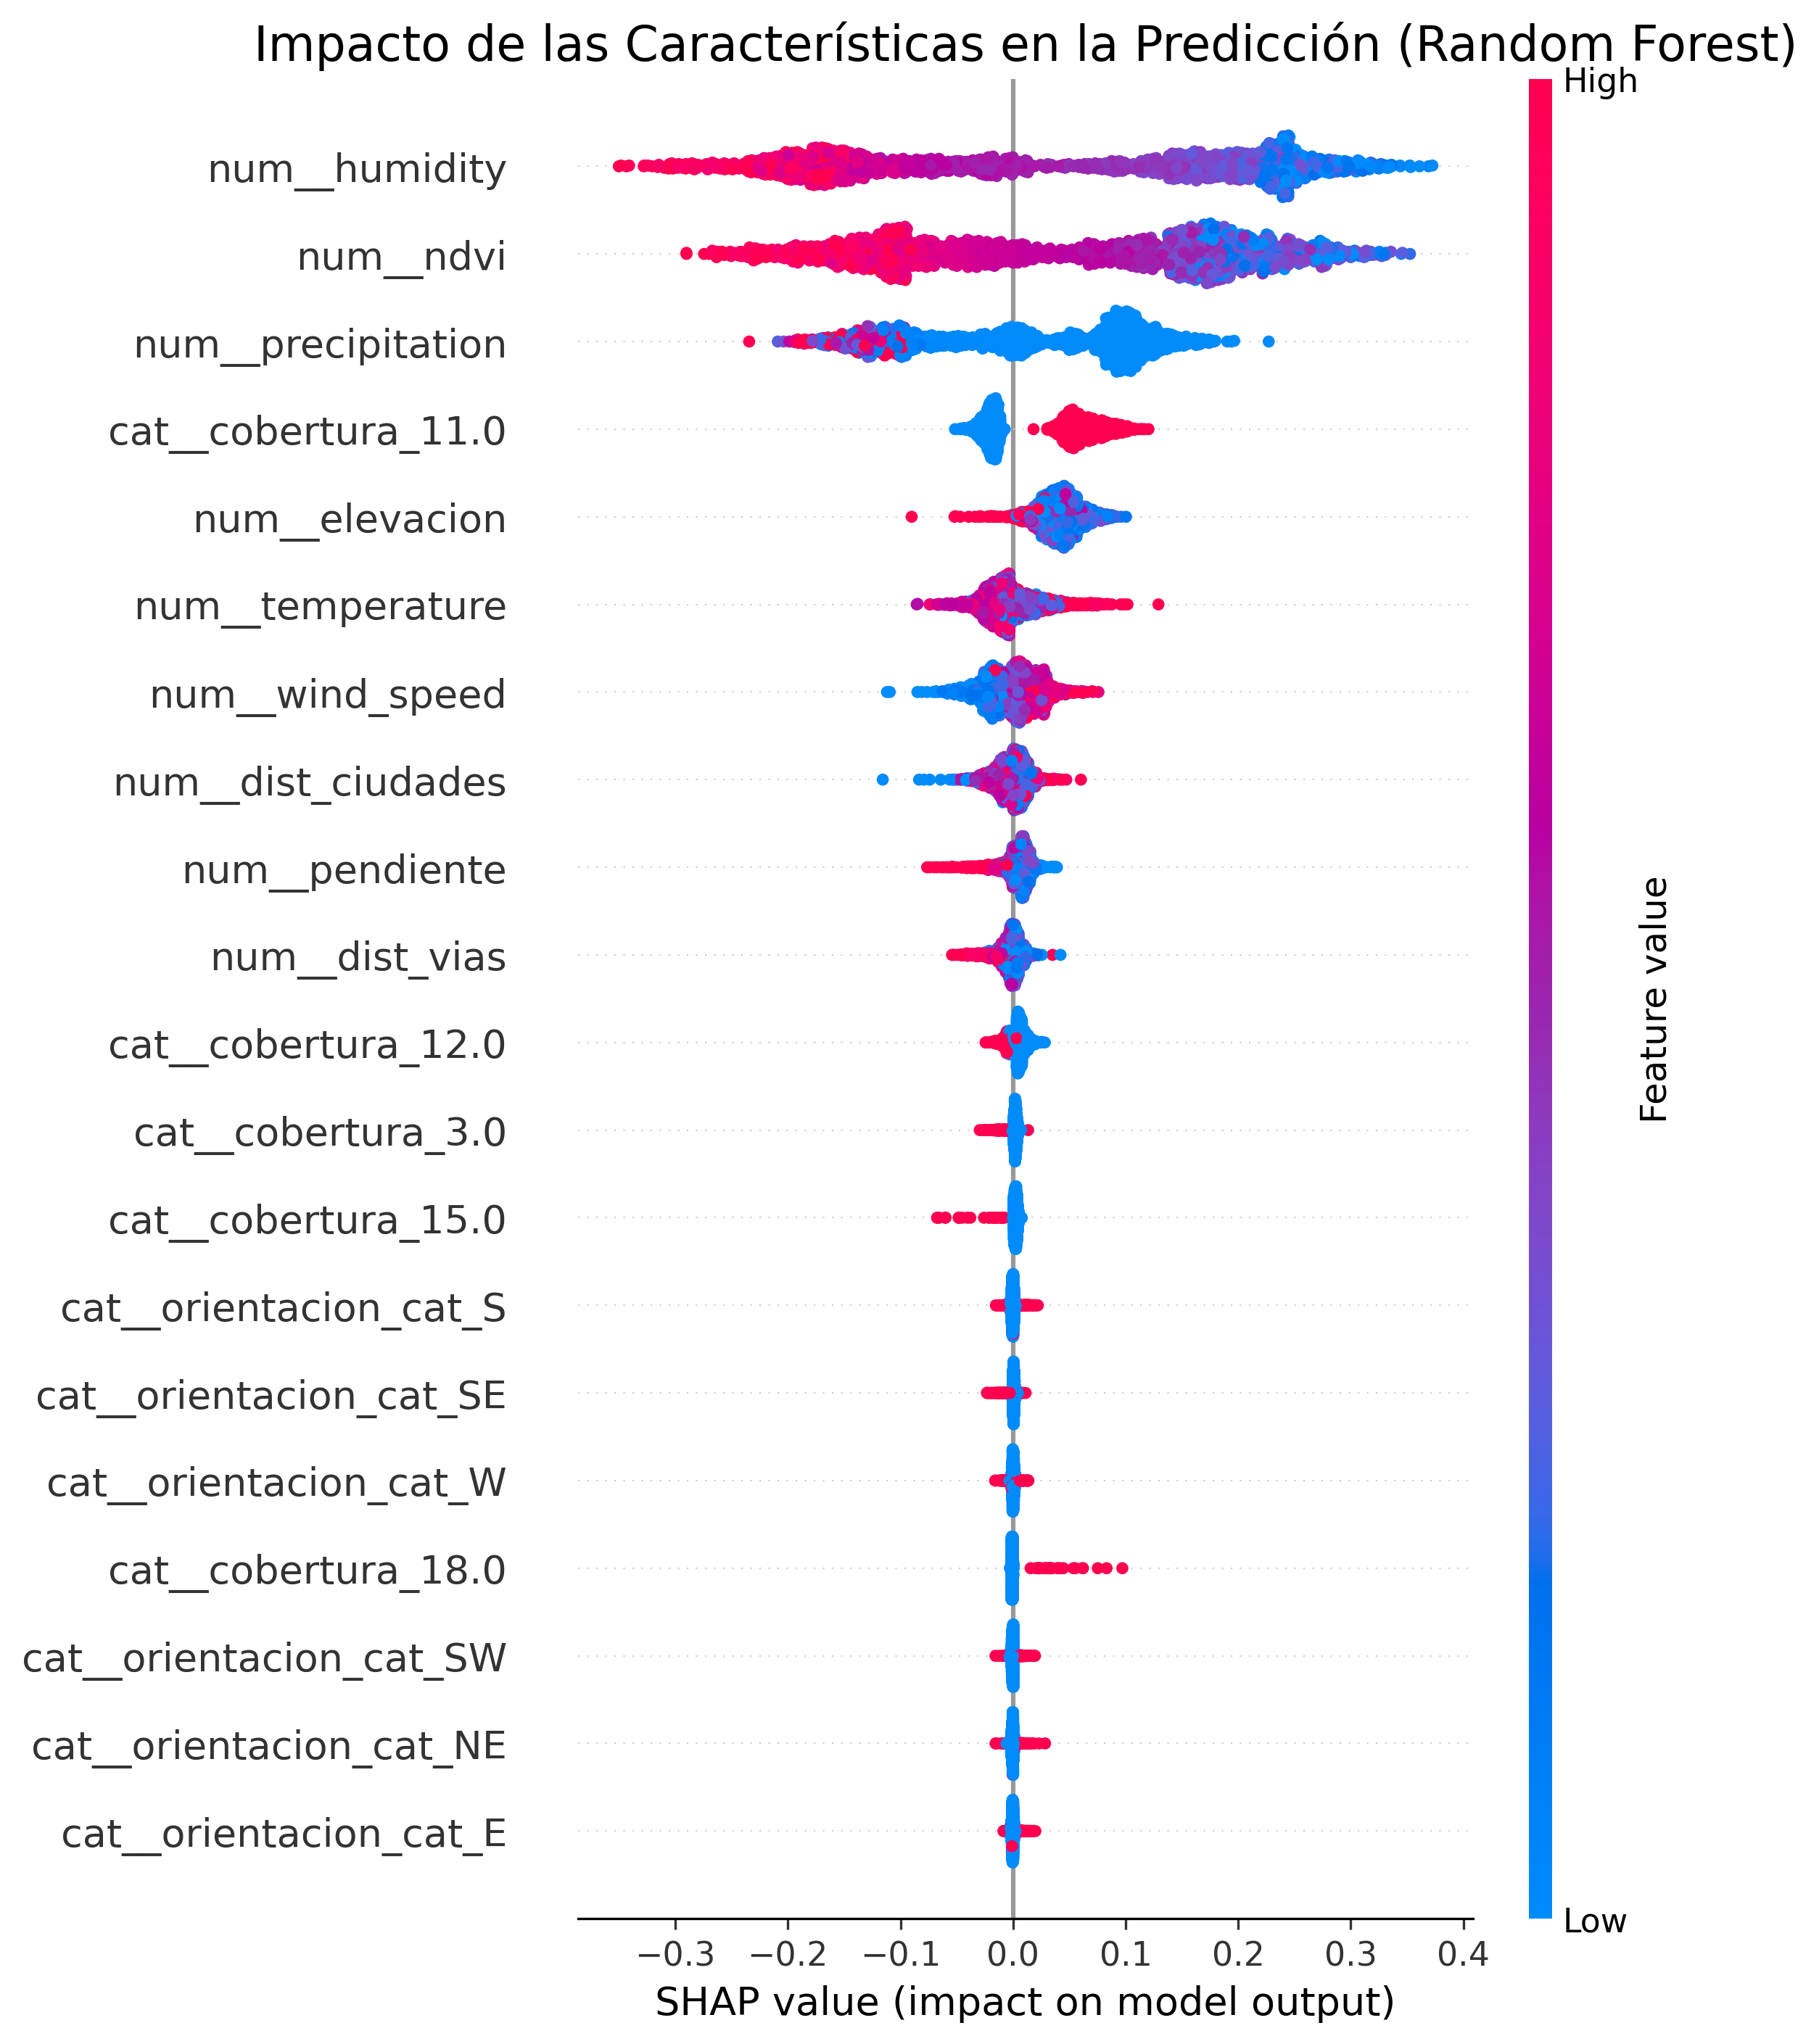
\includegraphics[width=\linewidth]{images/shap_summary_plot_rf.png}
    \caption{Gráfico de resumen SHAP (beeswarm plot). Cada punto es una predicción para una muestra. El color indica el valor de la característica (rojo=alto, azul=bajo) y su posición en el eje X indica su impacto en la predicción de incendio.Lado Positivo (Valor SHAP > 0): La característica, con su valor específico para esa muestra, aumentó la probabilidad de incendio.
Lado Negativo (Valor SHAP < 0): La característica, con su valor específico para esa muestra, disminuyó la probabilidad de incendio.}
    \label{fig:shap_summary}
\end{figure}
    

El gráfico de barras de importancia media confirma el ranking de las variables, promediando el impacto absoluto de cada una.
Este análisis no solo valida que el modelo está aprendiendo relaciones lógicas y esperadas (p.ej., más calor o cercanía a humanos aumenta el riesgo), sino que también proporciona información valiosa para los gestores de recursos, quienes pueden enfocar sus esfuerzos de prevención en las variables de mayor impacto.

\section{Aplicación Práctica: Generación del Mapa de Riesgo}
El objetivo final del pipeline es traducir el modelo predictivo en una herramienta visual y accionable. Para ello, se generó un mapa de riesgo de alta resolución para todo el departamento de Cordillera para una fecha específica

\subsection{Metodología de Generación}
El proceso para crear el mapa fue el siguiente:
\begin{enumerate}
    \item \textbf{Creación de una Rejilla de Predicción:} Se generó una rejilla o \textit{grid} de puntos uniforme que cubre toda la extensión del área de estudio.
    \item \textbf{Asignación de Variables a la Rejilla:} A cada punto de la rejilla se le asignaron todas las variables predictoras (topográficas, de cobertura, NDVI, de proximidad y climáticas para la fecha de interés) utilizando la misma función \texttt{asignar\_variables} usada para la muestra de entrenamiento.
    \item \textbf{Predicción de Probabilidad:} El pipeline de modelo entrenado se aplicó a esta rejilla enriquecida para predecir la probabilidad de incendio (un valor entre 0 y 1) para cada punto.
    \item \textbf{Interpolación y Visualización:} Los valores de probabilidad puntuales se interpolaron usando la función \texttt{griddata} para crear una superficie de riesgo continua. Esta superficie se visualizó como un mapa de calor (\textit{heatmap}), donde los colores cálidos (rojo) indican alta probabilidad de incendio y los colores fríos (amarillo/blanco) indican baja probabilidad.
\end{enumerate}

Este mapa es el producto más tangible del proyecto. Permite a los tomadores de decisiones identificar rápidamente los "puntos calientes" que requieren mayor vigilancia o la asignación prioritaria de recursos de prevención y combate, convirtiendo los datos y el modelo de Machine Learning en inteligencia accionable. Además, todas las predicciones puntuales se exportaron a un archivo \texttt{predicciones\_riesgo.csv} para su uso en otras plataformas o análisis.

\section{Algunos Conceptos}
\textbf{Semillas aleatorias:} Un número inicial utilizado para generar una secuencia de números pseudoaleatorios. Fijar una semilla asegura que cualquier proceso que involucre aleatoriedad (como la división de datos o el entrenamiento de ciertos modelos) produzca exactamente el mismo resultado cada vez que se ejecuta el código, garantizando la \textbf{reproducibilidad} del experimento.

\textbf{Rejilla (Grid):} Un conjunto de puntos distribuidos uniformemente sobre un área geográfica. Se usa como base para aplicar el modelo entrenado a toda la región y así poder generar un mapa de riesgo continuo.

\textbf{Geoespaciales vectoriales:} Datos que representan características geográficas mediante puntos, líneas y polígonos. En este proyecto, los límites del departamento, las ciudades y las vías son datos vectoriales.

\textbf{GeoDataFrame:} La estructura de datos fundamental de la librería \texttt{geopandas}. Es como un DataFrame de \texttt{pandas}, pero con una columna especial ("geometry") que almacena objetos geométricos, permitiendo realizar operaciones espaciales.

\textbf{Raster:} Un formato de datos geoespaciales que representa el espacio como una matriz de celdas o píxeles, donde cada píxel tiene un valor (ej. elevación, temperatura, clase de cobertura). El DEM y los mapas de NDVI son datos raster.

\textbf{Arreglos N-dimensionales etiquetados:} La estructura de datos principal de \texttt{xarray}. Permite almacenar datos multidimensionales (como un raster con coordenadas, tiempo y bandas) usando etiquetas (nombres de dimensiones y coordenadas) en lugar de índices numéricos, lo que facilita selecciones y operaciones complejas.

\textbf{Normalizar:} El proceso de escalar las variables numéricas para que estén en un rango común. Se hace para que las variables con magnitudes muy grandes (como la elevación en metros) no dominen a las de magnitudes pequeñas (como el NDVI) durante el entrenamiento del modelo.

\textbf{StandardScaler:} Una técnica de normalización de \texttt{scikit-learn} que transforma los datos para que tengan una media de 0 y una desviación estándar de 1.

\textbf{OneHotEncoder:} Un preprocesador que convierte variables categóricas (como "Norte", "Sur", "Este") en columnas binarias (0s y 1s), un formato que los modelos de Machine Learning pueden entender.

\textbf{Pipeline:} Un objeto de \texttt{scikit-learn} que encadena múltiples pasos de procesamiento y modelado en un solo flujo de trabajo. Asegura que la misma secuencia de transformaciones se aplique de forma consistente a todos los datos.

\textbf{Ensamble:} Una técnica de Machine Learning que combina las predicciones de varios modelos individuales (estimadores base) para producir una predicción final más precisa y robusta que la de cualquier modelo por sí solo. El Stacking es un tipo de ensamble.

\textbf{Meta-modelo:} En un modelo de Stacking, es el clasificador final que toma las predicciones de los modelos base como entrada y aprende a combinarlas de la mejor manera para dar el resultado definitivo.

\textbf{Calibrador (CalibratedClassifierCV):} Un wrapper de \texttt{scikit-learn} que se utiliza para ajustar las salidas de un modelo para que representen mejor una probabilidad real. Se usó sobre \texttt{LinearSVC} porque este no produce probabilidades de forma nativa.

\textbf{Boxplot (Diagrama de caja):} Una visualización estadística que representa la distribución de un conjunto de datos a través de sus cuartiles. Es útil para comparar rápidamente la mediana, la dispersión y los valores atípicos entre diferentes grupos.

\textbf{Heatmap (Mapa de calor):} Una visualización gráfica donde los valores de una matriz se representan como colores. Se usó para la matriz de confusión, donde los colores más intensos indican un mayor número de casos.

\textbf{Matriz de confusión:} Una tabla que resume el rendimiento de un modelo de clasificación. Compara las clases predichas con las clases reales y desglosa los resultados en verdaderos positivos, verdaderos negativos, falsos positivos y falsos negativos.

\textbf{Máscara de recorte (Clipping Mask):} Una forma o polígono utilizado para ocultar partes de otra capa visual. En el script, se usó el polígono del departamento para recortar el mapa de calor interpolado, asegurando que el riesgo solo se muestre dentro de los límites del área de estudio.

\textbf{Mapa de calor interpolado:} Una superficie continua de color creada a partir de valores en puntos discretos. La interpolación (como la cúbica) estima los valores en los espacios vacíos entre los puntos de la rejilla para crear una visualización suave y fácil de interpretar.

\textbf{Geometría poligonal:} Una forma vectorial cerrada que representa un área, definida por una secuencia de vértices conectados. El límite del departamento de Cordillera es una geometría poligonal.

\textbf{CRS (Coordinate Reference System):} Sistema de Coordenadas de Referencia. Es un estándar que define cómo las coordenadas de los datos geográficos se relacionan con lugares reales en la Tierra. Es crucial para asegurar que todas las capas de datos se alineen correctamente.

\textbf{Autocorrelación Espacial:} La propiedad inherente de los datos geográficos donde los valores de las mediciones en ubicaciones cercanas tienden a ser más similares que en ubicaciones lejanas. Es un factor clave a considerar en la validación de modelos espaciales.








\end{multicols}

\end{document}